\section{数据集制作问题与关键点}

\subsection{裁剪后文件命名}
文件命名时要注意高低分辨率影像对的匹配, 并且有唯一的id, 同时要体现数据来源. 最容易想到的命名方法是直接包含影像源ROI序号与行列号, 如图~\ref{fig:0201}所示:

\begin{figure}[!htbp]
    \centering
    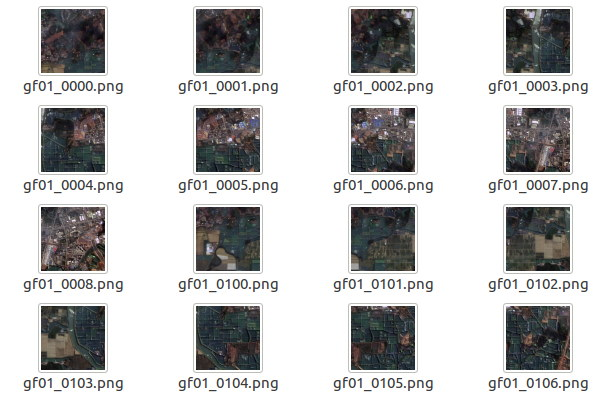
\includegraphics[height=15em]{pic/q0101.jpg}
    \caption{GF影像命名}
    \label{fig:0201}
\end{figure}

以高分影像为例, s=``gf01\_0304.png'', s[0:2]``gf''为影像数据源, 哨兵影像则为 ``s2'', 其表示哨兵2号; 之后的s[2:4]``01''表示裁剪的ROI序号为01, s[5:7]``03''表示裁剪的行号, s[7:9]``04''表示裁剪的列号.

影像裁剪主要依赖两个参数, 一是``sample\_size''裁剪大小, 在本次裁剪中使用的ROI为正方形, 为了有效利用ROI数据, 裁剪也使用正方形; 二是``sample\_step''裁剪步长, 用于控制每次裁剪小正方形移动的距离. 当 ``sample\_size''等于``sample\_step''时, 裁剪出的影像无重复区域.

对于每幅宽为$width$高为$height$的影像, 对与裁剪大小$sample\_size$, 裁剪步长$sample\_step$, 其可获得的裁剪影像数量$N$计算公式为:

\begin{equation}
    a = (height - sample\_size)\div sample\_step + 1 
\end{equation}

\begin{equation}
    b = (width - sample\_size)\div sample\_step + 1 
\end{equation}

\begin{equation}
    N = a * b
\end{equation}

\subsection{裁剪大小的平衡}
高分影像ROI分辨率为4000*4000, 哨兵影像分辨率为1000*1000. 第一次进行影像裁剪时, 高分影像选择的``sample\_size''为800, ``sample\_step''为400, 对应的哨兵影像``sample\_size''和``sample\_step''为200和100. 裁剪步长为裁剪大小的一半. 直接裁剪后共有$7*9*9=567$对影像. 经过人工剔除云雾后, 哨兵影像只有200幅左右, 数据量大减.
以高分影像为例, 部分有云雾遮挡如图~\ref{fig:0202}所示:

\begin{figure}[!htbp]
    \centering
    \subfloat[]{\label{fig:0202a}
    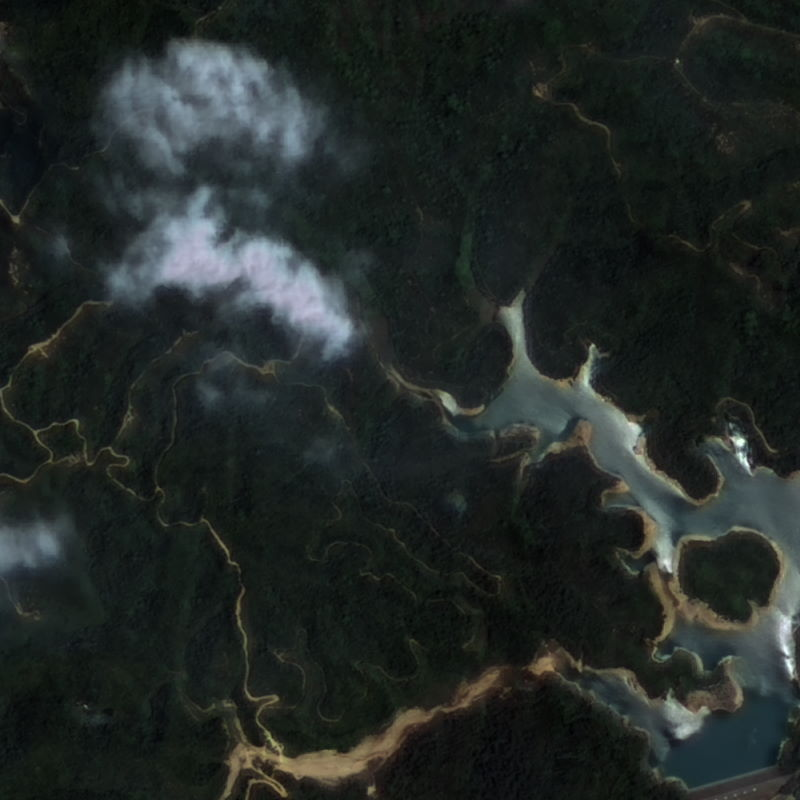
\includegraphics[height=10em]{pic/q0201.jpg}}
    \quad
    \subfloat[]{\label{fig:0202b}
    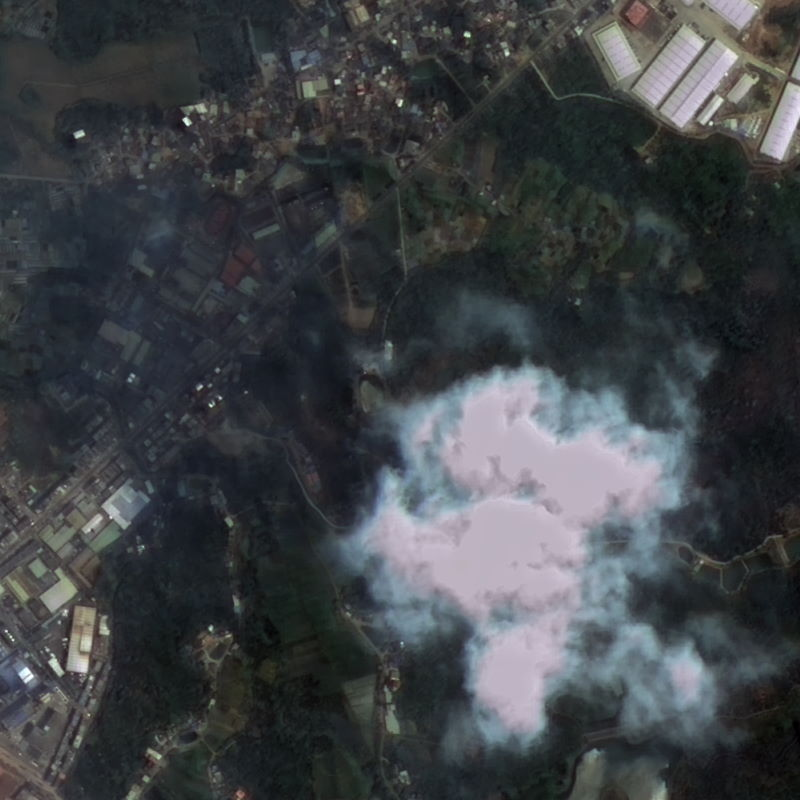
\includegraphics[height=10em]{pic/q0202.jpg}}
    \quad
    \subfloat[]{\label{fig:0202c}
    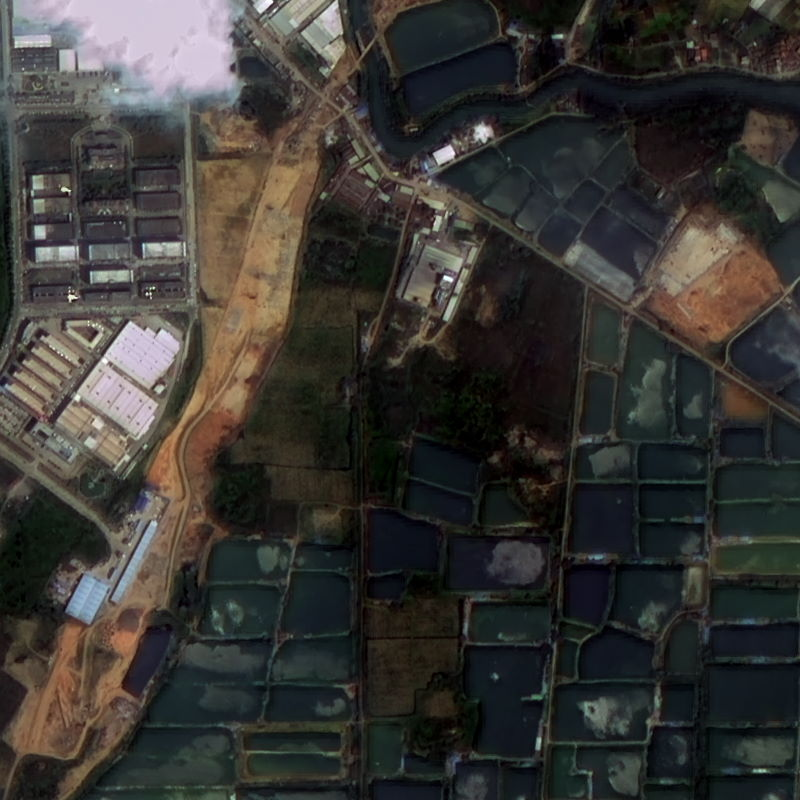
\includegraphics[height=10em]{pic/q0203.jpg}}
    \caption{GF影像裁剪结果}
    \label{fig:0202}
\end{figure}

在裁剪后的影像中, 部分云雾仅存在于影像的左上, 左下, 右上, 右下的小块中. 在下一步的人工剔除云雾时, 如果将此类影像剔除, 则会损失部分有效数据. 影像重叠虽可使云雾外数据得以在相邻裁剪影像中获得, 对于~\ref{fig:0202c}的云雾遮挡, 缩小``sample\_size''则会使有效数据增多. 

由于哨兵影像含有大量少云雾影像, 为提高影像利用率, 本次训练使用的GF数据裁剪大小为400, 裁剪步长为200. 对应哨兵影像裁剪大小与步长为100和50. 由此共得到$19*19*7=2527$对影像. 再对1000多幅影像进行了低质量剔除后, 再对共5000幅影像进行人工剔除云雾和变色的水田.  

但同时过多的重叠区域也需要警惕, 这意味着过多的重复数据, 对于训练来说, 不是好事情. 如图~\ref{fig:0203}所示, 蓝色为裁剪大小, 黑色为裁剪步长, 对本次裁剪步长为裁剪大小一半的情况来讲, 红色块代表最多重复4次的影像子块(ROI中间部分, 由于要剔除, 所以说最多), 黄色代表重复1次的影像子块(ROI四个角), 橙色代表重复2次的影像(ROI除角点的边). 即训练时过多重复数据, 同时加强影像内部权重, 等于没有加强, 而影像数量却增大4倍左右. 裁剪大小越小, 该现象越明显. 

\begin{figure}[!htbp]
    \centering
    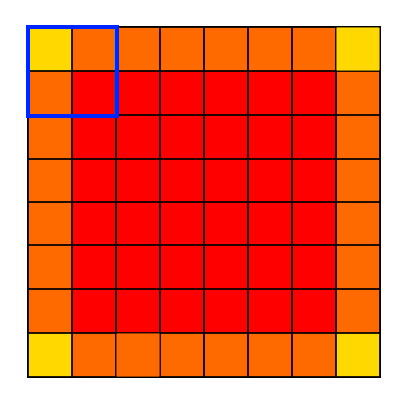
\includegraphics[height=12em]{pic/q0204.jpg}
    \caption{重叠区示意}
    \label{fig:0203}
\end{figure}

同时由于重叠区存在, 训练时的测试数据最好使用含少量云雾被剔除, 不在好数据集中的影像, 否则相当于测试数据属于训练数据子集. 

\subsection{云雾遮挡与水田变色}

\begin{figure}[!htbp]
    \centering
    \subfloat[gf]{\label{fig:0204a}
    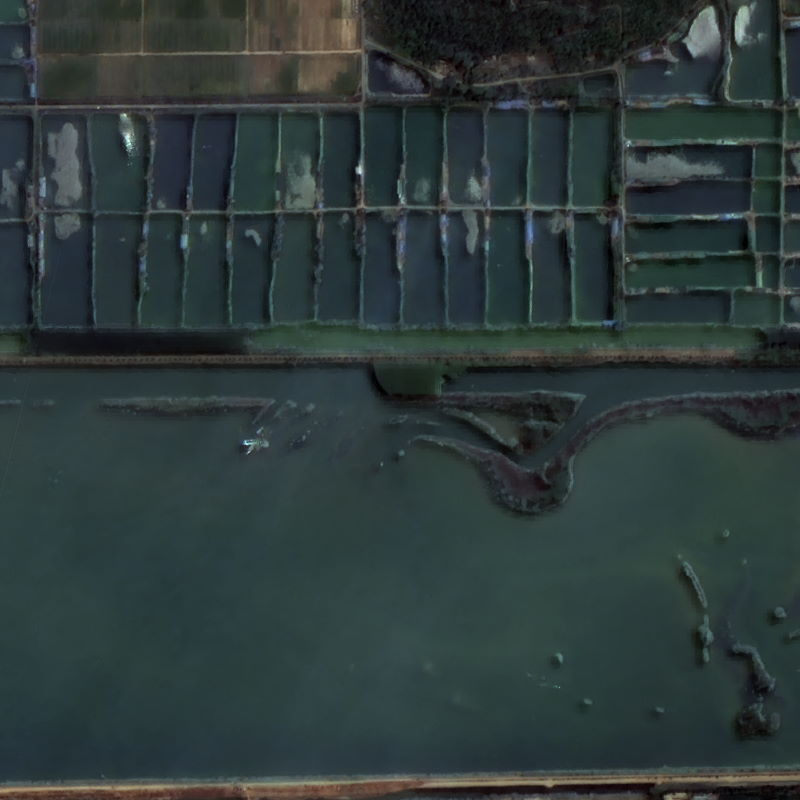
\includegraphics[height=10em]{pic/q0301.jpg}}
    \qquad
    \subfloat[s2直方图匹配后]{\label{fig:0204b}
    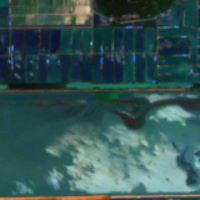
\includegraphics[height=10em]{pic/q0302.jpg}}
    \caption{水田差异}
    \label{fig:0204}
\end{figure}

除了光学遥感常见的云雾遮挡外造成影像对剔除外, 由于遥感影像拍摄于中国广东省东莞市和惠州市附近, 其水田较多. 不同时间(尽管只有一两周间隔)水田成像相差较大, 以``01\_0302''为例, 如上图~\ref{fig:0204}所示. 有可能是云倒影, 也有可能是河流中的泥沙. 此类数据也需剔除, 相比之下, 城市影像在两周之内, 变化较小. 经过人工剔除云雾遮挡和水田变色的低质图像后, 数据中城镇影像偏多, 这也是数据集要注意的一个问题.

\subsection{直方图匹配效果}
以高分影像裁剪大小800, 步长400为例. 其结果如图~\ref{fig:0205}和~\ref{fig:0206}所示.

\begin{figure}[!htbp]
    \centering
    \subfloat[s2]{\label{fig:0205a}
    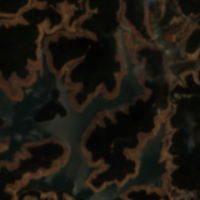
\includegraphics[height=10em]{pic/q0401lr.jpg}}
    \quad
    \subfloat[s2 matched]{\label{fig:0205b}
    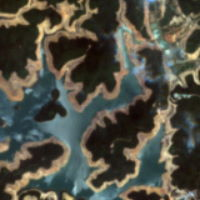
\includegraphics[height=10em]{pic/q0401lrm.jpg}}
    \quad
    \subfloat[gf]{\label{fig:0205c}
    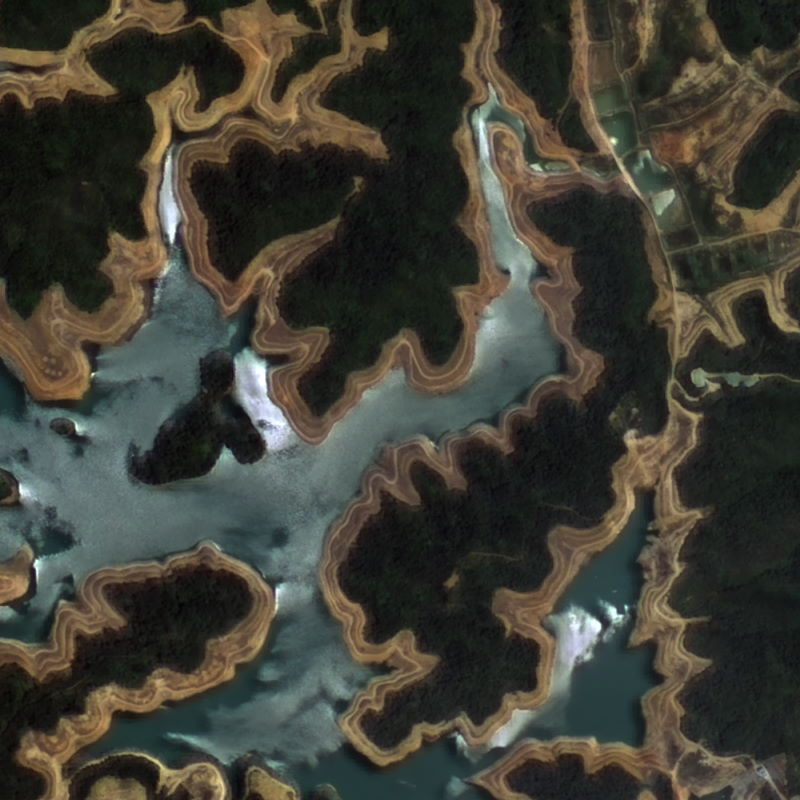
\includegraphics[height=10em]{pic/q0401hr.jpg}}
    \caption{030506结果}
    \label{fig:0205}
\end{figure}

\begin{figure}[!htbp]
    \centering
    \subfloat[s2]{\label{fig:0206a}
    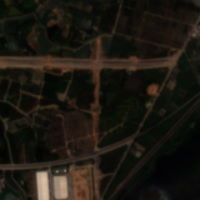
\includegraphics[height=10em]{pic/q0402lr.jpg}}
    \quad
    \subfloat[s2 matched]{\label{fig:0206b}
    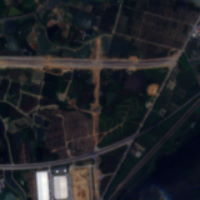
\includegraphics[height=10em]{pic/q0402lrm.jpg}}
    \quad
    \subfloat[gf]{\label{fig:0206c}
    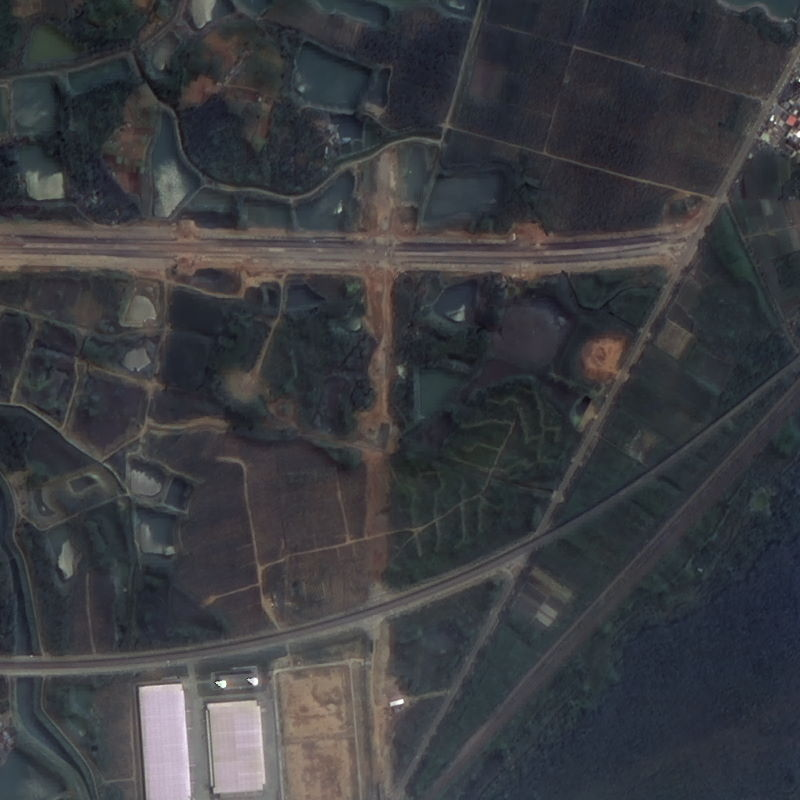
\includegraphics[height=10em]{pic/q0402hr.jpg}}
    \caption{070808结果}
    \label{fig:0206}
\end{figure}

直方图匹配后效果有显著提升, 匹配后哨兵影像和高分影像更加相似, 但还有一定差异.

% \begin{figure}[!htbp]
%     \centering
%     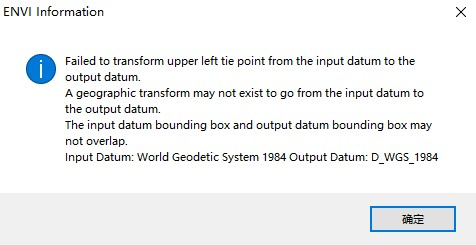
\includegraphics[height=10em]{pic/q0402.jpg}
%     \caption{ENVI重投影}
%     \label{fig:0217}
% \end{figure}


% \begin{figure}[!htbp]
%     \centering
%     \subfloat[]{\label{fig:0203a}
%     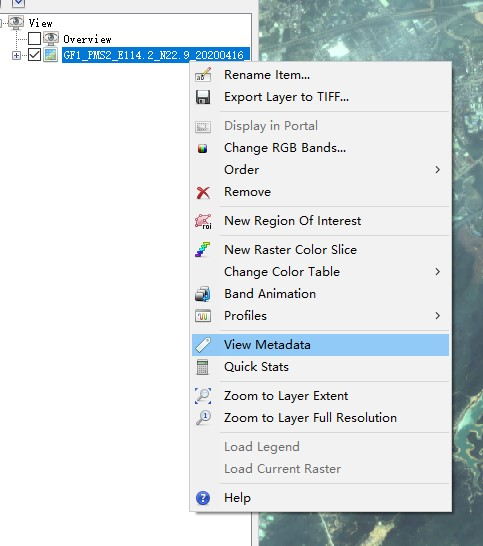
\includegraphics[height=12em]{pic/q1_02.jpg}}
%     \qquad
%     \subfloat[]{\label{fig:0203b}
%     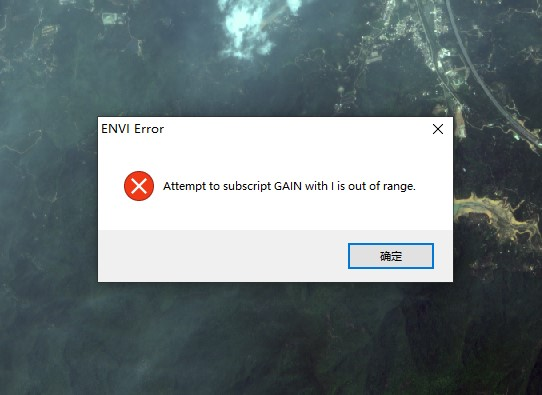
\includegraphics[height=12em]{pic/q1_04.jpg}}
%     \\[12pt]
%     \subfloat[辐射定标参数]{\label{fig:0203c}
%     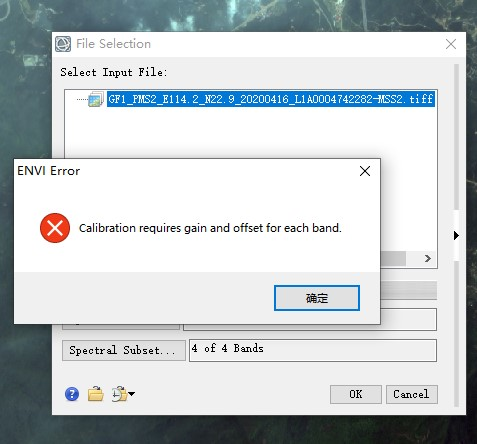
\includegraphics[height=12em]{pic/q1_03.jpg}}
%     \caption{元数据报错与辐射定标报错}
%     \label{fig:0203}
% \end{figure}

